\documentclass{report}
\usepackage[utf8]{inputenc}
\usepackage{amsmath}
\usepackage{graphicx}

\title{Eksamensnoter - Greedy Algorithms}
\author{André Oskar Andersen (wpr684)}
\date{\today}

\begin{document}
\maketitle

\section*{16 Greedy Algorithms}
\begin{itemize}
    \item A \textit{greedy algorithm} always makes the choice that looks best at the moment. That is, it makes a locally optimal choice in the hope that this choice will lead to a globally optimal solution.
\end{itemize}
\subsection*{16.1 An activity-selection problem}
\begin{itemize}
    \item Suppose we have a set $S = \{a_1, a_2, ..., a_n\}$ of $n$ proposed \textit{activities} that wish to use a resource, which can serve only one activity at a time. Each activity $a_i$ has a start time $s_i$and a finish time $f_i$, where $0 \leq s_i < f_i < \infty$. If selected, activity $a_i$ takes place during the half-open time interval $[s_i, fi)$. Activities $a_i$ and $a_j$ are compatible if the intervals $[s_i, f_i)$ and $[s_j, f_j)$ do not overlap. That is, $a_i$ and $a_j$are compatible if $s_i \geq f_j$ or $s_j \geq f_i$. In the \textit{activity-selection problem}, we wish to select a maximum-size subset of mutually compatible acitivites. We assume that the activites are sorted in monotonically increasing order of finish time: 
    $$f_1 \leq f_2 \leq f_3 \leq ... \leq f_{n - 1} \leq f_n$$
\end{itemize}
\textbf{The optimal substructure of the actiity-selection problem}
\begin{itemize}
    \item We can easily verify that the activity-selection problem exhibits optimal substructure. Let us denote by $S_{ij}$ the set of activities that start after activity $a_i$ finishes and that finish before activity $a_j$ starts. Suppose that we wish to find a maximum set of mutually compatible activities in $S_{ij}$, and suppose further that such a maximum set is $A_{ij}$, which includes some activity $a_k$. By including $a_k$ in an optimal solution, we are left with two subproblems: finding mutually compatible acitvities in the set $S_{ik}$ and finding mutually compatible activities in the set $S_{kj}$. Let $A_{ik} = A_{ij} \cap S_{ik}$ and $A_{kj} = A_{ij} \cap S_{kj}$, so that $A_{ik}$ contains the activities in $A_{ij}$ that finish before $a_k$ starts and $A_{kj}$ contains the activities in $A_{ij}$ that start after $a_k$ finishes. Thus, we have $A_{ij} = A_{ik} \cup {a_k} \cup A_{kj}$, and so the maximum-size set $A_{ij}$ of mutually compatible activities in $S_{ij}$ consists of $|A_{ij}| = |A_{ik}| + |A_{kj}| + 1$ activities
    \item The usual cut-and-paste argument shows that the optimal solution $A_{ij}$ must also include optimal solutions to the two subproblems for $S_{ik}$ and $S_{kj}$. If we could find a set $A'_{kj}$ of mutually compatible activities in $S_{kj}$ where $|A'_{kj}| > |A_{kj}|$, then we could use $A'_{kj}$ rather than $A_{kj}$, in a solution to the subproblem for $S_{ij}$. We would have constructed a set of $|A_{ik}| + |A'_{kj}| + 1 > |A_{ik}| + |A_{kj}| + 1 = |A_{ij}|$ mutually compatible activies, which contradicts the assumption that $A_{ij}$ is an optimal solution. A symmetric argument applices to the activies in $S_{ik}$.
\end{itemize}
\textbf{Making the greedy choice}
\begin{itemize}
    \item What do we mean by the greedy choice for the activity-selection problem? Intuition suggests that we should choose an activity that leaves the resource available for as many other acitivities as possible. Now, of the activities we end up choosing, one of them must be the first one to finish. Our intuition tells us, therefore, to choose the activity in \textit{S} with the earliest finish time, since that would leave the resource available for as many of the activities that follow it as possible.
    \item If we make the greedy choice, we have only one remaining subproblem to solve: finding activities that start after $a_1$ finishes. 
    \item Theorem 16.1 shows, that the greedy choice, in which we choose thefirst activity to finish, is always part of some optimal solution \\
    \item \textbf{Theorem 16.1}: Consider any nonempty subproblem $S_k$, and let $a_m$ be an activity in $S_k$ with the earliest finish time. Then $a_m$ is included in some maximum-size subset of mutually compatible activities of $S_k$
    \item \textbf{Proof of Theorem 16.1}: Let $A_k$ be a maximum-size subset of mutually compatible activities in $S_k$, and let $a_j$ be the activity in $A_k$ with the earliest finish time. If $a_j = a_m$, we are done, since we have shown that $a_m$ is in some maximum-size subset of mutually compatible activities of $S_k$. If $a_j \neq a_m$, let the set $A'_k = A_k - \{a_j\} \cup {a_m}$ be $A_k$ but substituting $a_m$ for $a_j$. The activities in $A'_k$ are disjoint,  which follows because the activities in $A_k$ are disjoint, $a_j$ is the first activity in $A_k$ to finish, and $fm \leq f_j$. Since $|A'_k| = |A_k|$, we conlude that $A'_k$ is a maximum-size subset of mutually compatible activities of $S_k$ and it includes $a_m$
\end{itemize}

\subsection*{16.2 Elements of the greedy strategy}
\begin{itemize}
    \item A greedy algorithm obtains an optimal solutin to a problem by making a sequence of choices. At each decision point, the algorithm makes the choice that seems best at the moment.
    \item How can we tell whether a greedy algorithm will solve a particular optimiation problem? No way works all the time, but the greedy-choice property and optimal substructure are the two key ingredients. If we can demonstrate that the problem has these properties, then we are well on the way to developing a greedy algorithm for it
\end{itemize}
\textbf{Greedy-choice property}
\begin{itemize}
    \item The first key ingredient is the \textit{greedy-choice property}: we can assemble a globally optimal solution by making locally optimal (greedy) choices. In other words, when we are considering which choice to make, we make the choice that looks best in the current problem, without considering results from subproblems
\end{itemize}
\textbf{Optimal substructure}
\begin{itemize}
    \item A problem exhibits \textit{optimal substructure} if an optimal solution to the problem contains within it optimal solutions to subproblems.
\end{itemize}

\subsection*{16.3 Huffman codes}
\begin{center}
    \item 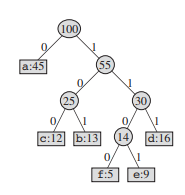
\includegraphics{../entities/huffman_binary_tree.png}
\end{center}
\begin{itemize}
    \item Huffman codes compress data very effectively. We consider the data to be a sequence of characters. Huffman's greedy algorithm uses a table giving how often each character occurs to build up an optimal way of representing each character as a binary string.
    \item Here, we consider the problem of designing a \textit{binary character code} (or \textit{code}) in which each character is represented by a unique binary string, which we call a \textit{codeword}.
    \item A \textit{variable-length code} gives frequent character short codewords and infrequent characters long codewords.
\end{itemize}
\textbf{Prefix codes}
\begin{itemize}
    \item We consider here only codes in which no codeword is also a prefix of some other codeword. Such codes are called \textit{prefix codes}
    \item Encoding is always simple for any binary character code; we just concatenate the codewords representing each character of the file.
    \item Prefix codes are desirable because they simplify decoding. Since no codeword is a prefix of any other, the codeword that begins an encoded file is unambiguous. We can simply identify the initial codeword, translate it back to the original character, and repeat the decoding process on the remainder of the encoded file.
    \item The decoding process needs a convenient representation for the prefix code so that we can easily pick off the initial codeword. A binary tree whose leaves are the given characters provides one such representation. We interpret the binary codeword for a character as the simple path from the root to that character, where 0 means "go to the left child" and 1 means "go to the right child".
    \item An optimal code for a file is always represented by a \textit{full} binary tree, in which every nonleaf node has two children. Since we can now restrict our attention to full binary trees, we can say that if $C$ is the alphabet from which the characters are drawn and all character frequencies are positive, then the tree for an optimal prefix code has exactly $|C| - 1$internal nodes.
    \item Given a tree $T$ corresponding to a prefix code, we can easily compute the number of bits required to encode a file. For each cahracter $c$ in the alphabet $C$, let the attribute $c.freq$ denote the frequency of $c$ in the file and let $d_T(c)$ denote the depth of $c$'s leaf in the tree. Note that $d_T(c)$ is also the length of the codeword for character $c$. The number of bits required to encode a file is thus
    $$B(T) = \sum_{c \in C} c.freg \cdot d_T(c)$$
    which we deine as the \textit{cost} of the tree $T$
\end{itemize}
\textbf{Constructing a Huffman code}
\begin{itemize}
    \item Huffman invented a greedy algorithm that constructs an optimal prefix code called a \textit{Huffman code}. Its proof of correctness relies on the greedy-choice property and optimal substructure.
\end{itemize}
\textbf{Correctness of Huffman's algorithm}
\begin{itemize}
    \item To prove that the greedt algorithm is correct, we show that the problem of determining an optimal prefix code exhibits the greedy-choice and optimal-substructure properties. The next lemma shows that the greedy-choice property holds.
\end{itemize}
\textbf{Lemma 16.2 (Greedy choice property)}
\begin{center}
    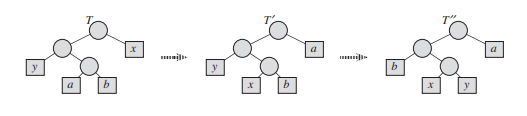
\includegraphics{../entities/fig_16_6.png}
\end{center}
\begin{itemize}
    \item Let $C$ be an alphabet in which each character $c \in C$ has frequency $c.freq$. Let $x$ and $y$ be two characters in $C$ having the lowest frequencies. Then there exists an optimal prefix code for $C$ in which the codewords for $x$ and $y$ have the same length and differ only in the last bit. \\
    \textbf{Proof}
    \begin{enumerate}
        \item The idea of the proof is to take the tree $T$ representing an arbitrary optimal prefix code and modify it to make a tree representing another optimal prefix code such that the characters $x$ and $y$ appear as sibling leaves of maximum depth in the new tree. If we can construct such a tree, then the codewords for $x$ and $y$ will have the same length and differ only in the last bit
        \item Let $a$ and $b$be two characters that are sibling leaves of maximum depth in $T$. Without loss of generality, we assumt that $a.freq \leq b.freq$ and $x.freq \leq y.freq$. Since $x.freq$ and $y.freq$ are the two lowest leaf frequencies, in order, and $a.freq$ and $b.freq$ are two arbitrary frequeincies, in order, we have $x.freq \leq a.freq$ and $y.freq \leq b.freq$.
        \item In the remainder of the proof, it is possible that we could have $x.freq = a.freq$or $y.freq = b.freq$. However, if we had $x.freq = b.freq$, then we would also have $a.freq = b.freq = x.freq = y.freq$, and the lemma would be trivially true. Thus, we will assume that $x.freq \neq b.freq$, which means that $x \neq b$
        \item We exchange the positions in $T$ of $a$ and $x$to produce a tree $T'$, and then we exchange the positions in $T'$ of $b$ and $y$ to produce a tree $T''$, in which $x$ and $y$ are sibling leaves of maximum depth. The difference in cost between $T$ and $T'$ is
        $$B(T) - B(T')$$
        $$ = \sum_{c \in C} c.freq \cdot d_T(c) - \sum_{c \in C} c.freq \cdot d_{T'} (c)$$
        $$ = x.freq \cdot d_T(x) + a.freq \cdot c_T(a) - x.freq \cdot d_{T'}(x) - a.freq \cdot d_{T'}(a)$$
        $$ = x.freq \cdot d_T(x) + a.freq \cdot d_T(a) - x.freq \cdot d_T(a) - a.freq \cdot d_T(x)$$
        $$ = (a.freq - x.freq)(d_T(a) - d_T(x))$$
        $$ \geq 0$$
        because both $a.freq - x.freq$ and $d_T(a) - d_T(x)$ are nonnegative.
        \item More specifically, $a.freq - x.freq$ is nonnegative because $x$ is a minimum-frequency leaf, and $d_T(a) - d_T(x)$ is nonnegative because $a$ is a leaf of maximum depth in $T$. Similarly, exchanging $y$and $b$ does not increase the cost, and so $B(T') - B(T'')$ is nonnegative. Therefore, $B(T'') \leq B(T)$, and since $T$is optimal, we have $B(T) \leq B(T'')$, which implies $B(T'') = B(T)$. This, $T''$ is an optimal tree in which $x$ and $y$ appear is sibling leaves of mximum dpeth, from which the lemma follows.
    \end{enumerate}
    \item Lemma 16.2 implies that the process of building up an optimal tree by mergers can, wihtout loss of generality, begin with the greedy choice of merging together those two characters of lowest frequency.
    \item The next lemma shows that the problem of constructing optimal prefix codes has the optimal-substructure property.
\end{itemize}
\textbf{16.3 (optimal-substructure property)}
\begin{itemize}
    \item Let $C$ be a given alphabet with frequency $c.freq$ defined for each character $c \in C$. Let $x$ and $y$ be two characters in $C$with minimum frequency. Let $C'$ be the alphabet $C$with the characters $x$ and $y$ removed and a new charahcter $z$ added. Define $freq$ for $C'$ as for $C$, except that $z.freq = x.freq + y.freq$. Let $T'$be any tee representing an optimal prefix code for the alphabet $C'$. Then the tree $T$, obtained from $T'$ by replacing the leaf node for $z$ with an internal node having $x$ and $y$ as children, represents an optimal prefix code for the alphabet $C$. \\
    \textbf{Proof}:
    \begin{enumerate}
        \item We first show how to express the cost $B(T)$ of tree $T$ in terms of the cost $B(T')$ of tree $T'$. For each chatacter $c \in C - \{x, y\}$, we have that $d_T(c) = d_{T'}(c)$, and hence $c.freq \cdot d_T(c) = c.freq \cdot d_{T'}(c)$. Since $d_T(x) = d_T(y) = d_{T'}(z) + 1$, we have 
        $$x.freq \cdot d_T(x) + y_freq \cdot d_T(y) = (x.freq + y.freq)(d_{T'}(z) + 1)$$
        $$ = z.freq \cdot d_{T'}(z) + (x.freq + y.freq)$$
        from which we conclude that  
        $$B(T) = B(T') + x.freq + y.freq$$
        or, equivalently
        $$B(T') = B(T) - x.freq - y.freq$$
        \item We now prove the lemma by contradiction. Suppose that $T$ does not represent an optimal prefix code for $C$. Then there exists an optimal tree $T''$ such that $B(T'') < B(T)$. Without loss of generality, $T''$ has $x$ and $y$ as siblings. Let $T'''$ be the tree $T''$with the common parent of $x$ and $y$ replaced by a leaf $z$ with frequency $z.freq = x.freq + y.freq$. Then
        $$B(T''') = B(T'') - x.freq - y.freq$$
        $$ < B(T) . x.freq - y.freq$$
        $$ = B(T')$$
        yielding a contradiction to the assumption that $T'$ represents an topimal prefix code for $C'$. Thus, $T$must represent an optimal prefix code for the alphabet $C$.
    \end{enumerate}
\end{itemize}

\end{document}